\documentclass[%
    12pt,
    ngerman,
    fleqn,
    parskip=half,
    DIV=15, BCOR=2cm, headinclude,
]{scrbook}


\usepackage{cite}


\usepackage{header}

\def\table{\def\figurename{Tabelle}\figure}
\let\endtable\endfigure 

\usepackage{csquotes}
\usepackage{booktabs}
\usepackage{algpseudocode}
\usepackage{placeins}

\usepackage{caption}

\usepackage{diagbox}

\usepackage{pdfpages}


%\usepackage[backend=biber,style=alphabetic]{biblatex}
%\addbibresource{Quellen.bib}


\usepackage{float}
\newfloat{algorithm}{tbhp}{loa}[chapter]
\floatname{algorithm}{Algorithmus}

\usepackage{tikz}
\usepackage{pgfplots}


\hypersetup{
    pdftitle={%
        Konstruktion, Aufbau und Inbetriebnahme eines Wirbelbetts zur Granulatfluidisierung
    }
}

\usepackage{datetime}
\usepackage{wallpaper}


\newcommand\bootstrapsamples{N_\text P}
\newcommand\gausswidth{\sigma}
\newcommand\initialrandomwidth{\tilde \Delta}
\newcommand\iterations{M}
\newcommand\iterationsbetween{M_\text{Zw}}
\newcommand\margin{\Delta}
\newcommand\mass{\mu}
\newcommand\preiterations{M'}
\newcommand\rounds{\bar n}
\newcommand\timesites{N}
\newcommand\timestep{a}

%\addto\captionsngerman{\renewcommand{\bibname}{}}


\subject{
	FH Aachen \\
	Fachbereich Energietechnik \\
	Studiengang Physikingenieurwesen
	}
\title{%
    Konstruktion, Aufbau und Inbetriebnahme eines Wirbelbetts zur Granulatfluidisierung
}
\subtitle{Bachelorarbeit}
\author{
    Vorgelegt im Jahr 2016 von Christoph Hansen \\
    \small{geboren am 30. April 1992 in Aachen} \\
    Zum Erlangen des akademischen Grades \\    
    \large{Bachelor of Engineering (B.Eng.)}
    }
    
\date{}    

\publishers{%
	Angefertigt am Institut für Materialpyhsik im Weltraum am Deutschen Zenstrum für Luft- und Raumfahrt, vorgelegt dem Fachbereich 10 der Fachhochschule Aachen, Campus Jülich
	
	\begin{figure}[h]
		\begin{center}
				
\includegraphics[scale=0.06]{DLR_Logo.png}
		\end{center}
	\end{figure}

}

\uppertitleback{%
    1. Prüfer: Prof. Dr.-Ing. Michael Stellberg \\
    2. Prüfer: Prof. Dr. Matthias Sperl 
}

\lowertitleback{%
	
	\small{
	Die vorliegende Arbeit ist bis zum 30.9.2017 streng vertraulich zu behandeln. Die Inhalte dieser Arbeit dürfen im oben genannten Zeitraum weder ganz, noch in Auszügen ohne Einwilligung der Firma Dritten zugänglich gemacht werden.
	Insbesondere darf die vorliegende Arbeit im genannten Zeitraum nicht in einer Bibliothek aufgestellt werden. Sie darf nur nach vorheriger Absprache mit Prof. Dr.-Ing. Michael Stellberg im Labor für Produktentwicklung der FH Aachen, Campus Jülich eingesehen werden.
	
	Die Weitergabe oder die Verwertung der Unterlagen, Informationen und/oder Kenntnissen ist ausnahmsweise zulässig, soweit dies zum ordnungsgemäßen Ablauf des Prüfungsverfahrens gemäß der Prüfungsordnung der FH Aachen erforderlich ist.
	}
	
	
	\vspace{2cm}
	
Ich versichere hiermit, dass ich die vorliegende Arbeit selbstständig verfasst und keine anderen als im Quellenverzeichnis angegebenen Quellen benutzt habe. Stellen, die wörtlich oder sinngemäß aus veröffentlichten oder noch nicht veröffentlichten Quellen entnommen sind, sind als solche kenntlich gemacht. Die Zeichnungen oder Abbildungen in dieser Arbeit sind von mir selbst erstellt worden oder mit einem entsprechenden Quellennachweis versehen. Diese Arbeit ist in gleicher oder ähnlicher Form noch bei keiner anderen Prüfungsbehörde eingereicht worden.
	
	\vspace{2cm}
	
	\hspace*{\fill}\begin{tabular}{@{}l@{}}\hline
		\makebox[6cm]{Christoph Hansen}
	\end{tabular}
	
	\vspace{2cm}
	
	Die Arbeit wurde betreut von: 
	
	\textcolor{white}{Das ist ein Platzhalter}

	\begin{minipage}{0.5\textwidth}
		
\includegraphics[scale=0.6]{FH_Aachen_Logo.png}
	\end{minipage}
	\begin{minipage}{0.5\textwidth}
		Prof. Dr.-Ing. Michael Stellberg
	\end{minipage}
	\begin{minipage}{0.5\textwidth}
		
\includegraphics[scale=0.04]{DLR_Logo.png}
	\end{minipage}
	\begin{minipage}{0.5\textwidth}
		Prof. Dr. Matthias Sperl
	\end{minipage}	
}




\begin{document}

%\maketitle

\includepdf[pages={1-5}, fitpaper=true]{FH_Aachen_Chris.pdf}

\CenterWallPaper{1}{Seitenhintergrund.png}

\setcounter{page}{1}

\tableofcontents

\newpage

\chapter{Einleitung}


\section{Einführung}

Bei fast allen Stoffen muss die Stofftemperatur ändern, damit sie in einen anderen Aggregatzustand wechseln. Bei granularen Medien ist das nicht nötig, stattdessen wird eine Säule des Mediums mittles unterschiedlich hoher Luftdurchsätze zu den verschiedenen Aggregatzustänge angeregt. \\
Da man bisher kein tiefgehendes Verständnis darüber hat welche Parameter sich wie auf die Entstehung der einzelnen Aggregatzustände auswirken, soll dies im Rahmen einer Doktorarbeit untersucht werden. \\
Ausgang war ein Aufbau eines Wirbelbettes, das allerdings nur begrenzt nutzbar war und sich auf Grund verschiedener Unzulänglichkeiten, nur für qualitative Messungen nutzen lies. \\
\hfill \\
Diese Arbeit behandelt die Neukonzeption des bestehenden Wirbelbettes am Deutschen Zentrum für Luft- und Raumfahrt, Institut für Materialphysik im Weltraum. Dabei geht es vor allen Dingen darum mit welchen konstruktiven Lösungen die Mängel des bisherigen Wirbelbettes behoben wurden. Weiterhin werden Testmessungen gemacht, um die Funktion des Wirbelbettes nachzuweisen.



\section{Grundlegende Begrifflichkeiten}

\subsection{Granulare Medien}

Unter Granulat versteht man ein Medium, das aus einzelnen harten Körnern besteht, die jeweils den Gesetzen der Newtonschen Mechanik unterworfen sind. Weiterhin haben die Körner eine Mindestgröße von $\SI{10}{\micro\meter}$, dabei spielt die Form der Oberfläche keine Rolle. Dies folgt aus der Forderung, das Schwingungen die Körner nicht mehr als ganzes anregen können sollen. \\
Ein weiteres Charakteristikum von Granulaten ist die Dissipertivität. Das heißt, dass die hauptsächlich kinetische Energie der Körner fast komplett in Wärmeenergie umgewandelt werden kann. Hier gilt die Energieerhaltung der klassischen Mechanik nicht. \\
Daraus ergibt sich als weiteres Merkmal granularer Medien die Sedimentation. Das bedeutet, das sich kleinere Partikel zwischen größeren bewegen können und so eine höhere Packungsdichte erreicht wird. \\
\hfill \\ 
Wie bei Molekülen gibt es auch bei granularen Medien ein dynamisches Verhalten. Dieses kann man hervorrufen, indem man mittels Schwingungen, also Vibration, auf das Granulat einwirkt. Man erhält dann ein schwingungsfluidiertes Granulat, in dem die Bewegung der Teilchen mit der Brownschen Molekularbewegung vergleichbar ist. \\
Die unterschiedlichen Energiezustände des Granulats werden gerne mit den Aggregatzuständen molekularer Stoffe verglichen:


\begin{center}
\begin{figure}[h]
	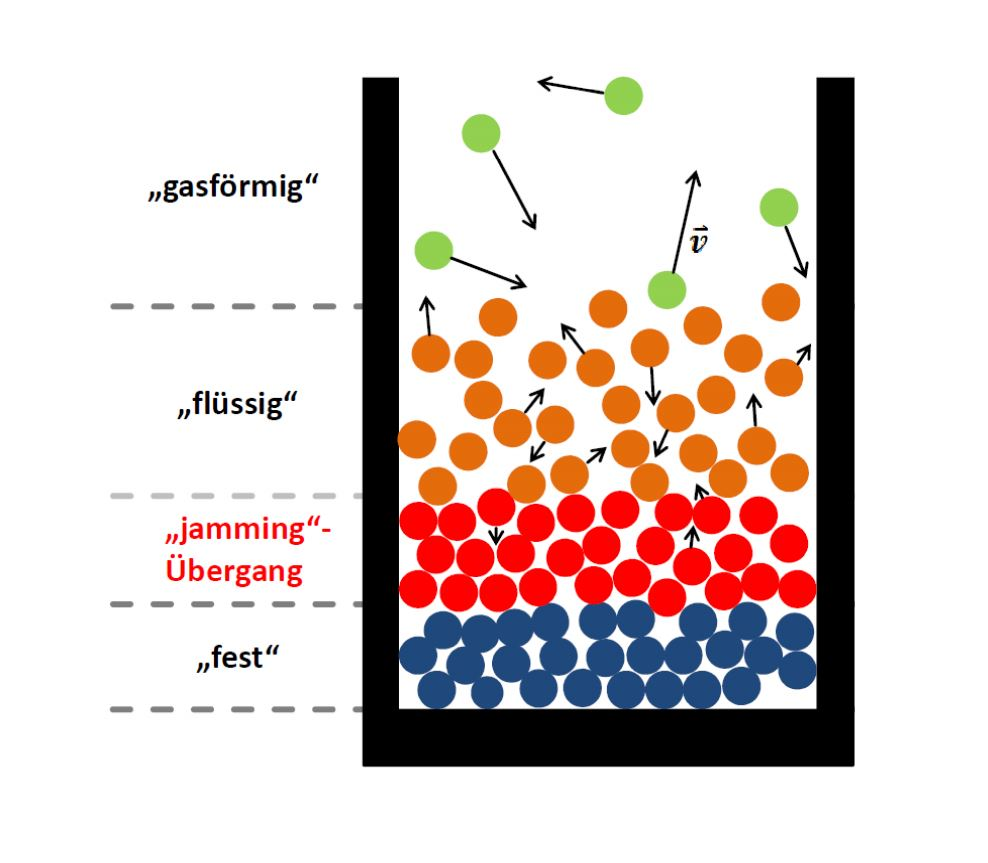
\includegraphics[scale=0.45]{Einleitung_1.jpg}
	\caption{Unterschiedliche Phasen eines Granulats}
\end{figure}	
\end{center}

Die in Abbildung 1.1 zu sehenden Phasen treten alle gleichzeitig während einer Anregung durch Vibration auf. \\
Im gasförmigen Zustand sind die Abstände der Partikel weit größer als der Partikeldurchmesser und die Partikel bewegen sich weitgehend unabhängig voneinander. \\
Der darunterliegende flüssige Zustand bietet bereits deutlich weniger Bewegungsfreiheit. Die mittlere freie Weglänge ist auf die Größenordnung der Partikel gesunken (fragen!). Man spricht auch von einem Glasübergang. \\
Charakteristisch für granulare Medien ist der \glqq jamming\grqq \ Übergang zwischen fest und flüssig. Hier ist keine Diffusion mehr möglich, die Partikel verbleiben also in ihrer Packungsposition und verklemmen mit ihrer Nachbarn. Bereits in diesem Zustand bilden sich sogenannte \glqq force chains\grqq \ heraus, über die die Kraftübertragung des Systems läuft. \\
Die \glqq force chains\grqq \ bilden sich im festen Zustand vollständig heraus und entstehen vor allem dadurch, das ein Teilchen deutlich mehr Nachbarn hat, als zu Stabilisation braucht. Da sich die Partikel amorph anordnen, verlaufen die \glqq force chains\grqq \ nicht homogen und isotrop, sondern willkürlich, was sich in einer unregelmäßigen Kraftverteilung ausdrückt.



\subsection{Ionisator}

Unter einem Ionisator versteht man ein Gerät, das ein Medium ionisiert und des dadurch elektrisch leitfähig macht. Je nach Bauweise und je nachdem wie das Gerät das Medium ionisiert, gibt es unterschiedliche Anwendungszwecke. \\
Ich beschränke mich hier auf einen Ionisator, der mittels eines starken elektrischen Feldes Luft ionisiert und unserem Anwendungszweck genügt. \\
Unser Ionisator besteht aus einem Netzteil, das $\SI{7}{\kilo V}$ Spannung erzeugt und einem Aufsatz, an dessen Ende ein elektrisches Feld zwischen der Metallspitze und dem äußeren Ring erzeugt wird.


Foto machen!!


\subsection{Flowcontroller}

Ein Flowcontroller ist ein Gerät mit dem man Flüsse gasförmiger oder flüssiger Medien kontrollieren kann. In der Regel kann ein Flowcontroller nur mit einem Aggregatzustand arbeiten und auch dort muss auf die verschiedenen Medien kalibriert werden, damit die angegeben Fehlergrenzen eingehalten werden. \\
Flowcontroller gibt es für viele verschiedene Flussraten, Genauigkeiten, Medien und Ansteuerungssysteme. Wie bei allen Produkten gilt auch hier das Prinzip, desto mehr Features, desto teurer der Controller. \\
Bei wissenschaftlichen Untersuchungen wie unserem Experiment kommt man um bestimmte Features nicht herum, da eine hohe Genauigkeit und präzises Ansteuern besonders wichtig sind. Dies wird im Abschnitt XXX genauer erläutert.



\section{Wissenschaftliche Fragestellung}

In der heutigen Zeit möchte man immer komplexere Metallteile am Stück formen, da dies, wegen weniger potentieller Bruchstellen, zu höherer Stabilität führt. Besonders ist man daran interessiert das jetzige Warmformgebungsverfahren bei hohlen Aluminiumprofilen auch für Stahlprofile nutzbar zu machen. \\
Dabei steht man vor der Herausforderung, das man bei den Temperaturen der Stahl Warmformgebung keine Ölmischung mehr nutzen kann, da sich diese entzünden würde. \\
Aus diesem Grund wählte man als Medium die Stoffklasse der granularen Medien aus. Diese bringen allerdings den Nachteil mit sich, das sie kompressiebel sind und die an einer Seite aufgebrachte Kraft sich nicht homogen und isotrop auf den Wänden verteilt. 
Man nimmt an, das die Art der Kraftverteilung durch drei Hauptparameter charakterisieren lässt. Zum einen ist das die Form der verwendeten Partikel, die Größe der Partikel und die Adhäsionskrafte der Partikel untereinander. \\
Diese drei Parameter kann man gesammelt betrachten, indem man die granularen Medien in einem Wirbelbett fluidisiert und misst ab wann die Medien in die flüssige Phase übergehen. Dadurch erreicht man eine Vergleichbarkeit der Medien untereinander und kann im Anschluss besser entscheiden welche Medien sich als Kraftüberträger eignen. \\


\section{Ziele der Arbeit}

In der Arbeit soll ein vorhandener Versuchsstand für quantitative Messungen optimiert werden und der Versuchsstand soll sowohl mit Luft als auch mit Wasser betrieben werden können. Im Praxisprojekt werden die Probleme des bisherigen Setups analysiert und eine entsprechende Lösung für das Medium Luft konstruiert. \\ 
Der Zeitraum der Bachelorarbeit beschäftigt sich mit der Konzeption in wie fern sich das Setup auf Wasserbetrieb umrüsten lässt und mit dessen Umsetzung. \\
Die Arbeit wurde dazu in folgende Arbeitspakete unterteilt:


\subsection{AP 1}

In einem ersten Schritt werden die Eckdaten den Projekts gesammelt und den Anforderungen zugeordnet. Zudem wird über die Materialwahl entschieden und eine Stückliste aller Kaufteile erstellt. Außerdem werden erste Lösungsansätze definiert, was wiederum in die Liste der Kaufteile einfließt.


\subsection{AP 2}

Die bisherige Elektronik liegt schutzlos und unübersichtlich neben dem Versuchsaufbau. Hier ist es erforderlich diese in sofern zu verpacken, das klar ist welche Anschlüsse für was gedacht sind und das ein eine einfache Transportierbarkeit gewährleistet ist.
Weiterhin muss ein A-D Wandler in die Schaltung integiert und angeschlossen werden.

\subsection{AP 3}

Zum Betrieb es Wirbelbettes ist ein Gaszustrom nötig, bei dem sich der momentane Gasstrom präzise zwischen $\SI{0}{\liter / \hour} - \SI{3000}{\liter / \hour}$ regeln und der dabei anliegende Druck messen lässt. Weiterhin soll eine Komponente zur Befeuchtung der Luft integriert werden, die variabel zu- und abgeschaltet werden kann. \\
Zudem muss soll das ganze System mechanisch stabil sein und transportabel sein. \\
Die Aufgabe besteht darin einen geeigneten Flowcontroller anzuschaffen, den Luftbefeuchter auszulegen und die Verrohrung entsprechend der Anforderungen zu wählen und umzusetzen.

\subsection{AP 4}

Das Wirbelbett ist die Hauptbaugruppe um die sich das Projekt dreht. In ihr befindet sich bei den Versuchen das granulare Medium und an ihr finden die optischen Messungen statt. \\
Hier besteht die Aufgabe in einer nahezu völligen Neukonstruktion, um das Bett für einen größeren Messraum nutzbar zu machen und auch einige neue Features hinzuzufügen.


\subsection{AP 5}

\subsection{AP 6}

\subsection{AP 7}























\chapter{Praxisteil}

\section{Elektronik}

\subsection{Anforderungen}

Bei der Elektronik gab es zwei verschiedene Bereiche: \\
In einem ersten Schritt sollte ein A-D Wandler gefunden werden, damit der vorhandene Drucksensor genauer ausgelesen werden kann. Zum Start es Projekts wurde der Drucksensor über das $\SI{10}{bit}$ breite analoge Interface des Arduino ausgelesen. Das ist für eine genaue Auswertung der Experimente zu wenig. Der Drucksensor hat einen Messbereich von (nachgucken) und gibt diesen auf $\SI{0}{} - \SI{10}{V}$ aus. Da der Arduino maximal $\SI{5}{V}$ als Eingangsspannung verarbeiten kann, wird die Spannung über einen Spannungsteiler auf $\SI{0} - \SI{5}{V}$ reduziert und dann eingelesen. Das entspricht einer Genauigkeit von $\SI{0,004}{V/bit}$, was einer Genauigkeit von XXX mbar/Volt entspricht. \\
\hfill \\
Als Resultat soll die gesamte Elektronik als \glqq Blackbox\grqq \ vorliegen, sodass man nach außen hin nur noch Anschlüsse hat, die klar gekennzeichnet sind. Dies soll in Form eines speziell angefertigten Gehäuses erledigt werden, das zudem auch noch rudimentären Schutz gegen Schmutz bietet.


\subsection{Umsetzung}

\subsubsection{Elektronik}

Der Arduino bietet einen sehr einfachen SPI Bus zum Anschluss von Modulen an. Darüber können die digitalen Outputdaten, der angesteckten Module ausgelesen werden, unabhängig davon wie hoch die Auflösung der Module ist. Auf Grund dieser Voraussetzungen wurde entschieden ein Modul für diesen Bus zu verwenden. \\
Rechnung für 16 bit einfügen!!!!!! \\
Es gibt verschiedene $\SI{16}{bit}$ A-D Wandler auf dem Markt, allerdings gibt es den hier ausgewählten (einfügen!!!!) bereits auf einer fertig montierten Platine, die direkt in den Arduino eingesteckt werden kann. Zudem gibt es zu der Platine eine recht gute Dokumentation. 


Schaltskizze!!!

\subsubsection{Gehäuse}




























\chapter{Bewertung und Ausblick}


\section{Bewertung}

In diesem Abschnitt soll der Erfolg der einzelnen Arbeitspakete kritisch hinterfragt werden, um Raum zur Optimierung aufzuzeigen. 

\subsection{Elektronik}

Rückblickend wurde die Komplexität der Elektronik unterschätzt, was dazu führte, das sehr lange unklar war welche Teile verwendet werden. Dadurch war es nicht möglich in dem geplanten Zeitfenster ein finales Gehäuse für die Elektronik zu designen. Da der Zeitaufwand für das Design dieses Teils allerdings nicht sehr hoch war, war es ohne Probleme möglich es am Ende des Projekts zu machen. In Zukunft wäre es besser solche Probleme entweder früher zu erkennen oder das Design von vorne herein ans Ende zu stellen. 

\subsection{Gassystem}

Der gewählte Filter erfüllt zwar alle gestellten Anforderungen, bringt aber einen Nachteil mit sich. Trotz planem Filter beim Aufkleben auf das Probenröhrchen, verformt sich dieser im Laufe der Nutzung plastisch. Das führt zu einem zusätzlichen heben und senken des graularen Mediums um bis zu \SI{3}{cm} (im Rährchen mit \SI{40}{mm}  Durchmesser). Dieses Verhalten ist unerwünscht, da sich die Granulate deswegen nicht komprimieren und dann auf ihr Verhalten untersuchen lassen.  

\subsection{Wirbelbett}

Die Konstruktion des Wirbelbetts erfüllt alle Anforderungen und verlief fast optimal. Lediglich gegen Ende musste, auf Grund der Umstellung von Plastik auf Metall, die Konstruktion in einigen Punkten abgeändert werden. Die Umstellung führte auch zu einer Gewichtserhöhung des Wirbelbetts, wodurch es nun nicht mehr ohne Gegengewicht vom Halter im Labor gehalten werden kann.
Im Vergleich mit der vorigen Version wurde ein hochwertiges und quantitativ verwendbares Wirbelbett gebaut.

\subsection{Nutzung des 3D Druckers}

Durch die Anforderung einen Ionisator im Aufbau unterzubringen, war es nicht möglich ein anderes Material außer Plastik zu verwenden. Zudem konnte eine andere Herangehensweise gewählt werden, statt klassischen Technischen Zeichnungen und FEM, wurde die Methode des evolutionären Druckens gewählt. Das sparte die aufwändigen Simulationen und erlaubte das Testen der designten Teile unter Realbedingungen. Der Nachteil dieser Methode ist neben den  Fehldrucken, die bei ca \SI{10}{\%} lagen, der Overhead an Teilen. Dadurch das man das selbe Teil in verschiedenen Evolutionsstufen druckt, ist man nicht sehr materialsparend. \\
Die Qualität der gedruckten Bauteile war durchweg hoch, besonders die Stabilität ist beachtlich, allerdings dauert es zwei, drei Drucke bis man seinen Modell am Rechner soweit angepasst hat, das der Drucker so druckt, wie man es beabsichtigt. Zudem ist der Drucker anfällig im Bezug auf den Druckuntergrund. Während des Projekts ist das Kaptontape auf der Heizplatte kaputtgegangen und ohne dieses Tape auf der Heizplatte, ist es nicht möglich Teile mit Durchmesser größer als \SI{40}{mm} mit flachem Boden zu drucken. Die Drucke bogen sich und waren somit ungeeignet für dichtende Zwecke eingesetzt zu werden. Weiterhin stellte sich im Rahmen der Messungen heraus, das der gedruckte Anschlusszylinder nicht luftdicht ist. Die genauen Ursachen sind nicht untersucht worden, allerdings werden die nicht optimal miteinander verschmolzenen Außenwände dabei eine große Rollen spielen.


\subsection{Zusammenfassung}

Abschließend kann gesagt werden, dass das Projekt sehr erfolgreich verlief. Es wurden alle Anforderungen erfüllt und es ist nun möglich Granulate quantitativ zu vermessen.
Im Verlauf der Konstruktion wurden viele neue Erkenntnisse über das Verhalten verschiedener Tools und Materialien gewonnen. Dies sollte genutzt werden, um bei zukünftigen Projekten in diesem Bereich genauer planen und Risiken und Problemstellen besser einschätzen zu können.




\section{Ausblick}

Der Ausblick ist zweigeteilt, im ersten Teil wird auf das konstruierte Wirbelbett eingegangen und im zweiten Teil über dessen Weiterentwicklung diskutiert. 

Wie bereits in der Bewertung erwähnt, gibt es noch Raum für Verbesserungen bei einzelnen Komponenten. Dies betrifft zum Beispiel den Filter, der entweder ersetzt oder durch konstruktive Maßnahmen am biegen gehindert werden sollte. In diesem Zusammenhang kann man sich auch nochmal mit der Integration eines Luftionisator beschäftigen, da dies ein interessantes Konzept ist, unser Ionisator allerdings entweder zu wenig Leistung hatte oder der Filter zu wenig Ionen durchließ.
Weiterhin wäre es interessant zu untersuchen, ob und wie es möglich ist die 3D gedruckten Teile luftdicht zu machen. Eine Möglichkeit die erwogen wurde, ist das tränken des gedruckten Teils in Epokzitharz. Bei einem Versuch mit Z-Bond 90 war die Behandlung nicht erfolgreich und der Luftduchfluss verschlechterte sich nochmal. Hier wäre es interessant herauszufinden welche Materialien für eine luftdichte Versiegelung in Frage kommen und wie das gedruckte Teil damit behandelt werden muss. Der Vorteil wäre ein deutlich leichteres Wirbelbett.

Die Weiterentwicklung des Wirbelbetts bestünde darin, es auch mit Wasser betreiben zu können. Dies hat den Vorteil, das durch den höheren Auftrieb des Granulats im Wasser und durch die höhere Viskosität des Wassers, deutlich weniger Strömungsmedium gebraucht wird. Im Gegensatz zu Luft mit bis zu \SI{3}{m^3/h}, braucht es dann unter \SI{1}{l/h} Wasser, um die Teilchen zu fluidisieren. Zudem hat man bei der Verwendung von Wasser kein Problem mit Elektrostatik.
Der Nachteil von Wasser als Strömungsmedium besteht darin, das man eine Rückführung braucht und das Wasser im Kreislauf auch sauber gehalten werden muss.



\phantomsection
\addcontentsline{toc}{chapter}{Abbildungsverzeichniss}

\listoffigures




\phantomsection
\addcontentsline{toc}{chapter}{Literaturverzeichnis}


\bibliography{Quellen}
\bibliographystyle{unsrt}






\phantomsection
\addcontentsline{toc}{chapter}{Anhang}


\chapter*{Anhang}

\pagestyle{plain}

\section*{Literatur}

Die Literaturquellen, bis auf das zitierte Buch, befinden sich auf Grund des Umfangs auf der beigefügten DVD im Ordner \glqq Literatur\grqq .

\clearpage

\section*{Tabellen}

\begin{figure}[h!]  
	\captionabove{Gewindetabelle}
	\begin{center}
		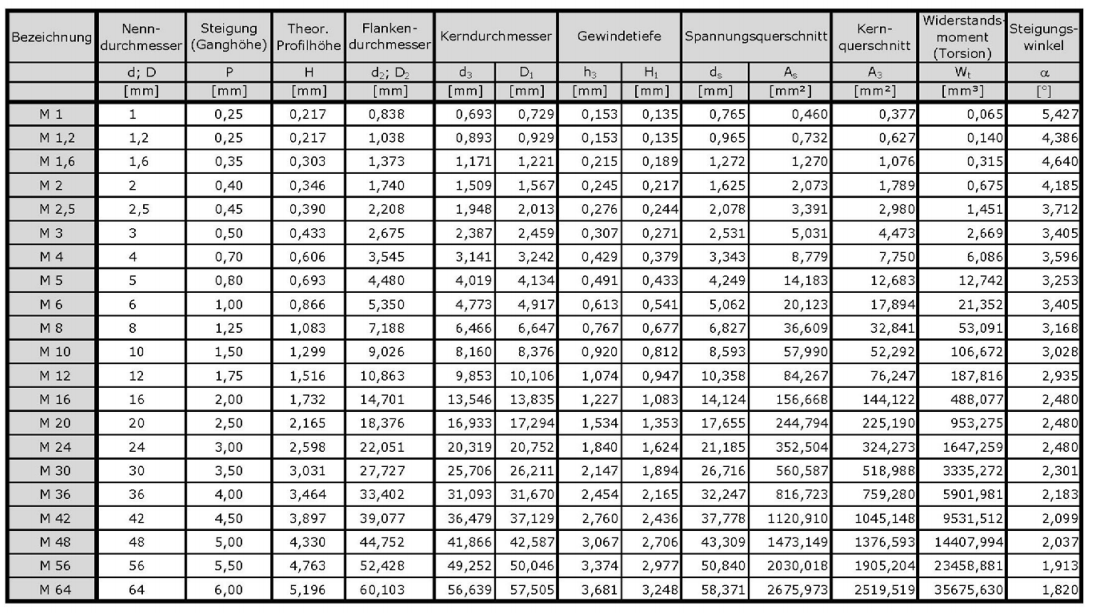
\includegraphics[page=1, scale=0.7, angle=90]{Anhang/Gewindetabelle.png}	
	\end{center}
\end{figure}

\clearpage

\section*{Technische Zeichnungen}

Im folgenden sind technische Zeichnungen zu allen Teilen aufgeführt, die für den Aufbau des designten Wirbelbetts benötigt werden.


\captionsetup{listof=false}

\begin{figure}  
	\captionabove{Halter oben 5mm}
	\includegraphics[page=1, scale=0.9, angle=90]{Anhang/Halter_oben_5mm.pdf}
\end{figure}

\begin{figure}  
	\captionabove{Halter oben 20mm}
	\includegraphics[page=1, scale=0.8, angle=90]{Anhang/Halter_oben_20mm.pdf}
\end{figure}

\begin{figure}  
	\captionabove{Halter oben 30mm}
	\includegraphics[page=1, scale=0.8, angle=90]{Anhang/Halter_oben_30mm.pdf}
\end{figure}

\begin{figure}  
	\captionabove{Halter oben 40mm}
	\includegraphics[page=1, scale=0.7, angle=90]{Anhang/Halter_oben_40mm_Blatt__1.pdf}
\end{figure}

\begin{figure}  
	\includegraphics[page=1, scale=0.8, angle=90]{Anhang/Halter_oben_40mm_Blatt__2.pdf}
\end{figure}

\begin{figure}  
	\captionabove{Schanierarm}
	\includegraphics[page=1, scale=0.7, angle=90]{Anhang/Schanierarm.pdf}
\end{figure}

\begin{figure}  
	\captionabove{Anschlusszylinder}
	\includegraphics[page=1, scale=0.8, angle=90]{Anhang/Anschlusszylinder_Blatt__1.pdf}
\end{figure}

\begin{figure}  
	\includegraphics[page=1, scale=0.8, angle=90]{Anhang/Anschlusszylinder_Blatt__2.pdf}
\end{figure}

\begin{figure}  
	\captionabove{Trichter 5mm}
	\includegraphics[page=1, scale=0.8, angle=90]{Anhang/Trichter_5mm.pdf}
\end{figure}

\begin{figure} 
	\captionabove{Trichter 20mm} 
	\includegraphics[page=1, scale=0.8, angle=90]{Anhang/Trichter_20mm.pdf}
\end{figure}

\begin{figure}
	\captionabove{Trichter 30mm}  
	\includegraphics[page=1, scale=0.8, angle=90]{Anhang/Trichter_30mm.pdf}
\end{figure}

\begin{figure}  
	\captionabove{Trichter 40mm}
	\includegraphics[page=1, scale=0.8, angle=90]{Anhang/Trichter_40mm.pdf}
\end{figure}

\begin{figure}  
	\captionabove{Swagelokrohrhalter}
	\includegraphics[page=1, scale=0.8, angle=90]{Anhang/Swagelokrohrhalter.pdf}
\end{figure}

\begin{figure}  
	\captionabove{Swagelokrohrhalter 2}
	\includegraphics[page=1, scale=0.8, angle=90]{Anhang/Swagelokrohrhalter2.pdf}
\end{figure}

\begin{figure}  
	\captionabove{Befeuchter Spirale}
	\includegraphics[page=1, scale=0.8, angle=90]{Anhang/Spirale_Befeuchter.pdf}
\end{figure}

\begin{figure}  
	\captionabove{Röhrchenhalter 5mm}
	\includegraphics[page=1, scale=0.8, angle=90]{Anhang/Halter_5mm.pdf}
\end{figure}

\begin{figure}  
	\captionabove{Röhrchenhalter 20mm}
	\includegraphics[page=1, scale=0.8, angle=90]{Anhang/Halter_20mm.pdf}
\end{figure}

\begin{figure}  
	\captionabove{Röhrchenhalter 30mm}
	\includegraphics[page=1, scale=0.8, angle=90]{Anhang/Halter_30mm.pdf}
\end{figure}

\begin{figure}  
	\captionabove{Röhrchenhalter 40mm}
	\includegraphics[page=1, scale=0.8, angle=90]{Anhang/Halter_40mm.pdf}
\end{figure}


\clearpage


\section*{Angebote und Rechnungen}

\includepdf[pages={1-2}, scale=0.9]{Anhang/Brooks_Flowcontroller_Angebot.pdf}

\includepdf[pages={1-2}, scale=0.9]{Anhang/O-Ringe1_Angebot.pdf}

\includepdf[pages={1-2}, scale=0.9]{Anhang/O-Ringe2_Angebot.pdf}

\includepdf[pages={1}, scale=0.9]{Anhang/Rechnung_Amazon_Nylonnetz.pdf}







\end{document}